\documentclass[border=8pt]{standalone}
\usepackage{ctex}
\usepackage{amsmath}
\usepackage{amssymb}
\usepackage{tikz}
\usetikzlibrary{arrows.meta}

\begin{document}
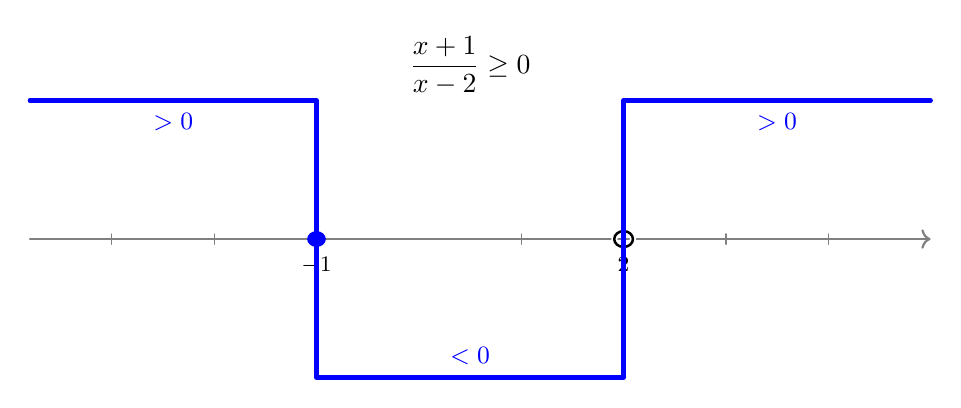
\begin{tikzpicture}[xscale=1.3, yscale=1.1, line cap=round, line join=round]

% 数轴
\draw[->, gray, line width=0.8pt] (-3.8,0) -- (5.0,0);
\foreach \x in {-3,-2,-1,1,2,3,4} \draw[gray] (\x,0.06) -- (\x,-0.06);

% 根：-1 实心（可取），2 空心（分母零点，不可取）
\fill[blue] (-1,0) circle (2.6pt);
\draw[white, line width=2.2pt] (2,0) circle (2.6pt);
\draw[black, line width=0.9pt] (2,0) circle (2.6pt);

\node[below=3pt, font=\footnotesize] at (-1,0) {$-1$};
\node[below=3pt, font=\footnotesize] at (2,0) {$2$};

% L 形穿根折线：右上起笔，依次穿过 2、-1
\draw[blue, line width=1.6pt]
  (5.0,1.6) -- (2,1.6) -- (2,-1.6) -- (-1,-1.6) -- (-1,1.6) -- (-3.8,1.6);

% 标注
\node[blue, font=\small] at (3.5,1.35) {$>0$};
\node[blue, font=\small] at (0.5,-1.35) {$<0$};
\node[blue, font=\small] at (-2.4,1.35) {$>0$};

\node[font=\normalsize] at (0.5,2.0) {$\dfrac{x+1}{x-2}\geq 0$};

\end{tikzpicture}
\end{document}
